\documentclass{article}
\usepackage[latin1]{inputenc}
\usepackage{enumerate}
\usepackage{hyperref}
\usepackage{graphics}
\usepackage{graphicx}
\usepackage{caption}
\usepackage{subcaption}
\usepackage{tabularx}
\usepackage{amsmath}
\newcommand{\ket}[1]{\ensuremath{\left|#1\right\rangle}}
\newcommand{\bra}[1]{\ensuremath{\left\langle#1\right|}}
\newcommand{\braket}[2]{\ensuremath{\left\langle #1 \middle| #2 \right\rangle}}
\newcommand{\obar}[1]{\ensuremath{\overline{ #1 }}}
% enumerate is numbered \begin{enumerate}[(I)] is cap roman in parens
% itemize is bulleted \begin{itemize}
% subfigures:
% \begin{subfigure}[b]{0.5\textwidth} \includegraphics{asdf.jpg} \caption{} \label{subfig:asdf} \end{subfigure}
\hypersetup{colorlinks=true, urlcolor=blue, linkcolor=blue, citecolor=red}
\graphicspath{ {C:/Users/Evan/Desktop/} }
\title{Assignment 3: \\ Introduction to \emph{Mathematica}\\
\large \emph{Introduction to Data Analysis for Physics}}
\author{Evan Ott and Will Beason}
\date{Spring 2014}
\setcounter{secnumdepth}{0}
\usepackage[parfill]{parskip}
\begin{document}
\maketitle
\section{Submission Requirements}
Submit the assignment to \href{mailto:data.analysis.physics@gmail.com}{data.analysis.physics@gmail.com} by Wednesday at 5pm. Just submit the \emph{Mathematica}
document you create (typically a .nb file).

\section{Problem 1}
For this problem, we'll look at how to inject intuition into \emph{Mathematica} to make it be able to solve problems more easily. You will benefit from some basic calculus knowledge.

\subsection{a}
Let's try to calculate $$\int_0^1x^adx$$ where $a$ is an arbitrary number. If we try this in \emph{Mathematica}, we get a conditional expression. Why? What would happen if
we set $a\leq-1$? (for this one, yes, I want English)

\subsection{b}
How about if we wanted to calculate $$\lim_{x\rightarrow\infty}x^r$$ for some $r$. What can we tell \emph{Mathematica} so that we can evaluate the limit? (you can just show me this time)

\subsection{c}
In the first homework, when you calculated $f(g(x))$, this did not evaluate immediately to just $x$, but instead $1 + \frac{1}{2}(-2+2x)$. The \texttt{Simplify} and \texttt{FullSimplify}
functions can simplify expressions, and are particularly helpful when you can apply some assumptions (look in the \emph{Mathematica} documentation to see some
examples). Create an example where these simplification functions cannot fully simplify the expression without applying some outside information (\texttt{x > 2} or \texttt{Element[y,Reals]}
or similar), then show what it simplifies to when you do apply the background information. ``Awesome points'' for finding such an expression that changes the end value based on the
assumption made, but with multiple simple solutions.

\section{Problem 2}
For this problem, you'll need the data at \url{http://www.cs.utexas.edu/~evanott/PHY110C_Textbook/static/data_analysis/_downloads/assignment3data.csv} (9 MB). This is data
for a simple (read: bad) gravity simulation for the Sun, Halley's Comet, the 8 planets, and Pluto (the 9th planet and everyone knows it). The first column is a time, then, in groups
of 3, is the x, y, and z coordinates of each of the objects (not necessarily in the order above).

\subsection{a}
Find a way to determine which object is which. In my case, I made a manipulable plot that showed the position of each particle at the time I wanted. I also fixed the plot range so that
I was always looking at the same range of coordinates as I manipulated time. For reference, see Figure \ref{fig:orbit}. Big hint: all 9 planets are listed consecutively from Mercury to Pluto.

\subsection{b}
The masses of the objects (in kg) are (in order of Halley's Comet, Mercury, Venus, ... Pluto, Sun):

\begin{verbatim}
{2.2*10^14, 3.3022*10^23, 4.869*10^24, 5.9722*10^24, 6.39*10^23, 1.8988*10^27, 
5.685*10^26, 8.6625*10^25, 1.0278*10^26, 1.324*10^22, 1.989*10^30}
\end{verbatim}

Using this, can you calculate the net momentum at the start (first two timesteps which are in seconds) of the simulation (x, y, z are in meters)? Furthermore, test other times to see if total momentum has
been conserved (2-3 additional points throughout the simulation is sufficient). 

To figure out the instantaneous momentum of one object relative to the reference frame we're in (arbitrary
selection of origin with Cartesian coordinates), we want to look at the difference in position between two timesteps $\Delta{\vec{x}}=(x_2-x_1, y_2-y_1, z_2-z_1)$ then find the
velocity by $\vec{v}=\frac{\Delta{\vec{x}}}{\Delta{t}}$ and non-relativistic momentum as $\vec{p}=m\vec{v}$. We'll total the momentum of the system by adding the vectors for
each object together. You may compare the direction or magnitude (or both) of the momentum to make your judgment about the simulation.

\begin{figure}
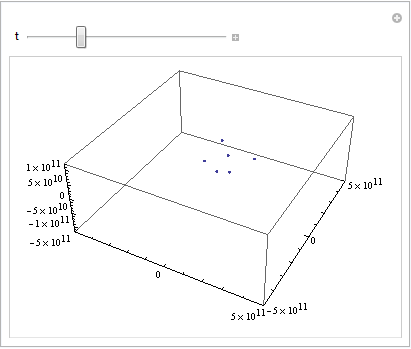
\includegraphics[scale=.85]{orbit.png}
\caption{Objects in orbit. (Don't worry, we'll make pretty graph extractions. This one is just low-resolution for space)}
\label{fig:orbit}
\end{figure}

\end{document}